% status: 10
% chapter: TBD

\title{GraphQL Web APIs}

\author{Averill Cate, Jr}
\orcid{1234-5678-9012}
\affiliation{%
  \institution{The University of Indiana}
  \streetaddress{}
  \city{Bloomington} 
  \state{Indiana} 
  \postcode{47408}
}
\email{acate@iu.edu}

\author{Gregor von Laszewski}
\affiliation{%
  \institution{Indiana University}
  \streetaddress{Smith Research Center}
  \city{Bloomington} 
  \state{IN} 
  \postcode{47408}
  \country{USA}}
\email{laszewski@gmail.com}

% The default list of authors is too long for headers}
\renewcommand{\shortauthors}{A. Cate}

\begin{abstract}
  This project is for Advanced Cloud Computing, Indiana University
  Spring Semester 2018.  Through this project, we will demonstrate the
  use of GraphQL and cloud computing   services as a means for constructing 
  and delivering web services.  The project will rely on The Santa Rita 
  Experimental Range (SRER) website and data sets maintained by the 
  Univeristy of Arizona and second, related web site, the Walnut Gulch 
  Experimental Watershed (WGEW) Online Data Access, maintained by the United 
  States Department of Agriculure's, Agriculure Research Service (ARS).  
  Neither of these existing sites provide modernized data services, yet both 
  sites provide potentiall valuable data to the research community.
\end{abstract}

\keywords{hid-sp18-505, GraphQL, Web, Services}

\maketitle

\section{Introduction}
What is GraphQL?  GraphQL is a query language for web application
programer interfaces (APIs)\cite{hid505FacebookGraphQL2018}.  There
have been been many other tools and methods used to develop APIs in
the past.  Some of those older tools are XML and SOAP, JSON and REST,
plain old text or comma separated files.  What makes GraphQL so
different?  First, as the name implies, GraphQL, is a query language.
This is different compared to SOAP/XML and Swagger/REST in that those
tools are a combination of data format and transport protocol.

Typically, SOAP/XML and Swagger/REST APIs are structured so that the
API user needs to review the specifications for interacting with the
API.  For example, what functions or endpoints are available?  What
are the parameters for those functions and what data types apply to
each parameter?  GraphQL is different in that it provides a mechanism
where an API becomes a domain specific language (DSL).  This means
that API consumers can focus on developing transactions with the API
based on the data domain of the API.  For example, a GraphQL API for
stock data would allow API users to format queries something like the
following:

\begin{verbatim}
{
   all_stocks {
     symbol, price, date
}
\end{verbatim}

In this example we see a query request to a GraphQL API that is asking 
for all stock data with respective symbol, price, an date.  
Alternatively, a REST based query might look like the following:

\begin{verbatim}
http://server.host.com/api/v1/allstocks
\end{verbatim}

In the REST based request we see information related to where the data
are being requested from, the protocol used to make the request, the
API version and finally, what the request is really after, all stock
data.  The latter could be considered more understandble to
programmers or even to someone who is technically a advanced web
users, but compared to the REST request, the GraphQL based request has
a format more closely resembling the data intself and is less concered
with how the data are requested.

A useful way to demonstrate the uses of GraphQL would be to apply
GraphQL to the development of a real-world API that will transform
existing web-based data sources created and maintained at United
Stated Deparment of Agriculture web site and the University of
Arizona.  The first data resource is the Santa Rita Experimental which
is an experimental range currently maintained by the University of
Arizona.  The experimental range was the first of its kind and was
established in 1902\cite{hid505SrerWebSite2018}.  The SRER website, in
its current state, is not structured to deliver data as a service.
The second data source is the Walnut Gulch Experimental Watershed,
which is also an outdoor research facility located in southestern
Arizona\cite{WgewWebSite2018}.  Like the SRER site, the WGEW
preicpitation and runoff data site is not structured to delivered as
services.

\subsection{General Outline}

\begin{enumerate}
\item Web scraping existing data source to download, parse and clean
  existing data.
\item Load the data into a database.
\item Develop a small web application to provide two web services.
  The two services will deliver the same data.  However, one of the
  services will use GraphQL\cite{hid505FacebookGraphQL2018} to deliver
  data and the other will use REST\cite{hid505swaggerio2018} to
  deliver its data.
\item Develop a simple load testing tool that will be used to
  determine performance metrics for both services and compare the
  results of the load tests.
\item Time permitting, create a simple Amazon Lambda service that will
  compute some metric related to the preciption/runoff data.  The
  purpose is to demonstrate how cloud services can be used to off-load
  costs and dependencies on a distributed system like the one proposed
  in this project.
\item Time permitting, develop a 3-node Raspberry Pi cluster to host
  the application.  The purpose of this, is to demonstrate how a
  system like this one can be hosted and deployed on hardware
  infrastructure that is cheap and relatively simple to maintain.
\end{enumerate}

\section{Data Collection}

Data were collected from the Santa Rita Experimental Range website.  In 
Figure~\ref{f:srer_landing_page}, we see the present day landing 
page for SRER.  What is not apparent in the landing page is the 
plethora of data available data available in the site.

\begin{figure}[htb]
  \centering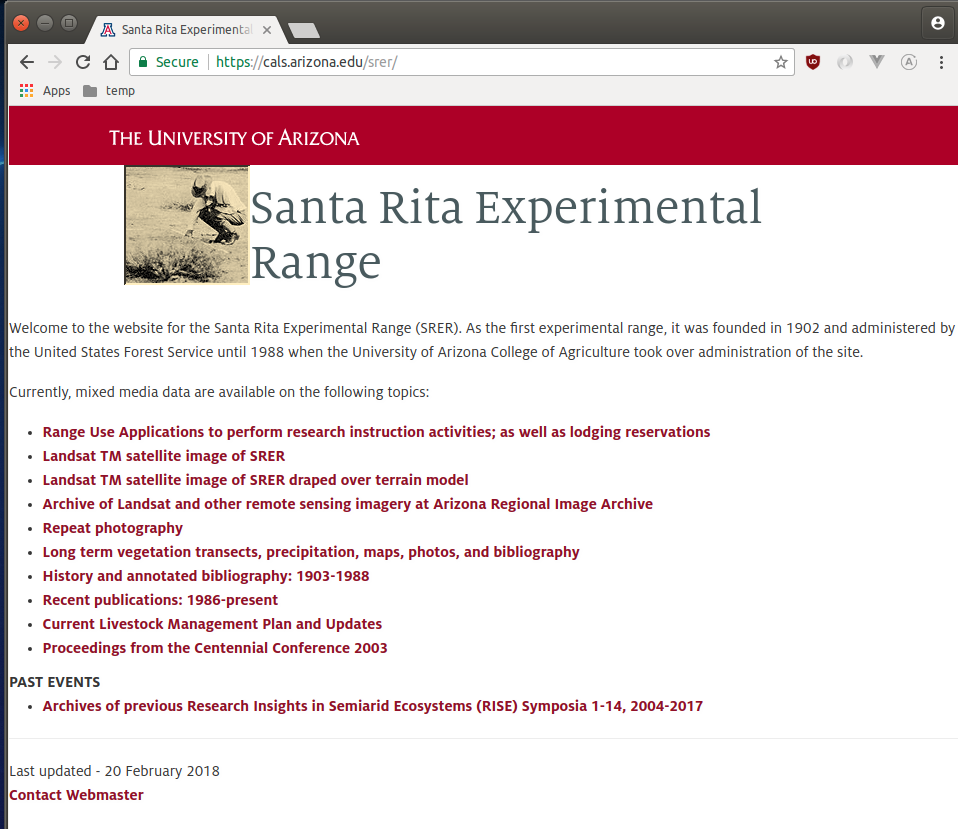
\includegraphics[width=\columnwidth]{./images/srerlandingpage.png}
  \caption{SRER Page\cite{hid505SrerWebSite2018}}\label{f:srer_landing_page}
\end{figure}


In Figure~\ref{f:srerprecipdata} we have navigated one page deeper into 
the SRER site and as can be seen, meta-data and data are both availabe, but as 
raw text files.  These data are consumable as is, but could be enhanced by 
being made machine readible by creating web services to deliver the data.

\begin{figure}[htb]
  \centering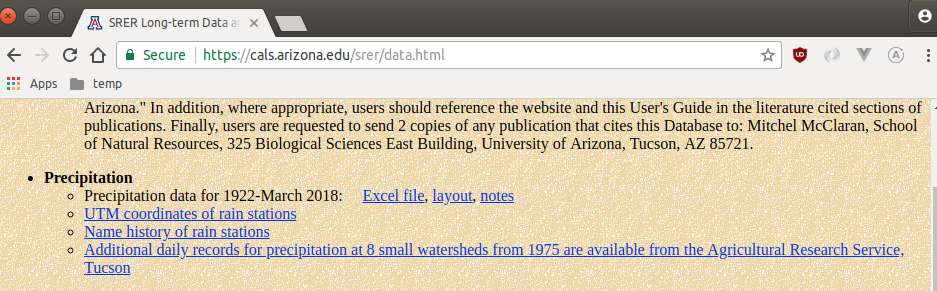
\includegraphics[width=\columnwidth]{./images/srerprecipdata.png}
  \caption{SRER Precip.\cite{hid505SrerWebSite2018}}\label{f:srerprecipdata}
\end{figure}

\section{Data Loading}
The data sets downloaded for this demonstration were the raingage Universal 
Transverse Mercator (UTM) coordinate data files and the Excel file that 
contained all of the preciption data for the respective raingages.  Some of 
the raingage data had to be cleaned mostly due to typographical errors and the 
UTM coordinates had to be converated to latitude and longitude values in case 
the data are rendered in mapping applications.

The precipitation data had to be converted from an Excel file to a CSV file 
and the value delimiter was changed from a comma to the pipe symbol.  The 
reason for this is because the comma can occur in some of the descriptive text 
data for raingages, where as the pipe symbol is typically not used in written 
English.

\section{Web API Development}
After the data were prepared for import into a database, the foundation for a 
simple web API application was established using the following software:

\begin{enumerate}
  \item Docker - a container platform\cite{hid505Docker2018}
  \item Python - the programming language
  \item Graphene - a Python programming language library that is used to 
  develop GraphQL APIs
  \item PostgresQL - the database server
  \item Django - a Python based model-view-controller (MVC) web development 
  framework
  \item Django Rest Framework - a Django plugin that facilitates the 
  development of REST APIs
  \item Graphene Django - a Django plugin that facilitates development of 
  GraphQL APIs
\end{enumerate}

\subsection{REST/Swagger API}
Generally, a REST based API endpoints, in combination with a tool like Swagger 
are combined to create a web interface like the one shown in 
Figure~\ref{f:rest_swagger_ui}.  The figure provides an example of the various 
API endpoints (e.g., /api/srer/v1.0/precipevents).  Some endpoints require 
input parameters which are used to execute parameterized queries (e.g., 
queries that filter data) data, while other endpoints require no parameters 
and typically return a list of data entities.

\begin{figure}[htb]
  \centering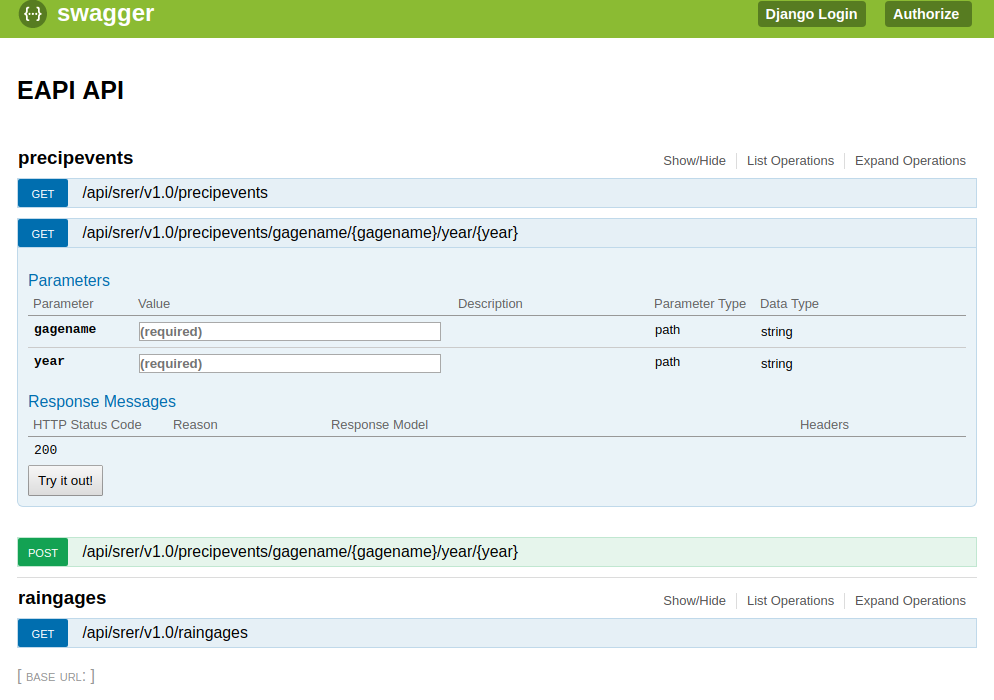
\includegraphics[width=\columnwidth]{./images/rest_swagger_ui.png}
  \caption{REST/Swagger UI}\label{f:rest_swagger_ui}
\end{figure}

In Figure~\ref{f:srer_rest_raingage_list} we see an example of a REST 
request's response and the resulting JSON data packet.  The JSON request is 
relatively clear.  Based on the request url in 
Figure~\ref{f:srer_rest_raingage_list} we know the domain name (localhost), 
API context (srer), API version number (v1.0) and the data being requested 
(raingages).  However, in a REST API unless well documented by the developers, 
developing properly formated parameterized request urls can be challenging.  
However, the difficulties are counter-balanced by the implementing a Swagger 
UI for the API and making sure proper documentation is added, so the end-user 
has as much information as possible.

The JSON response is a bit more intuitive.  From firgure 
Figure~\ref{f:srer_rest_raingage_list} we can see the basic data structure and 
data types.  There are many programming libraries that automate the parsing of 
JSON data into domain objects that facilitate API client development.

\begin{figure}[htb]
  \centering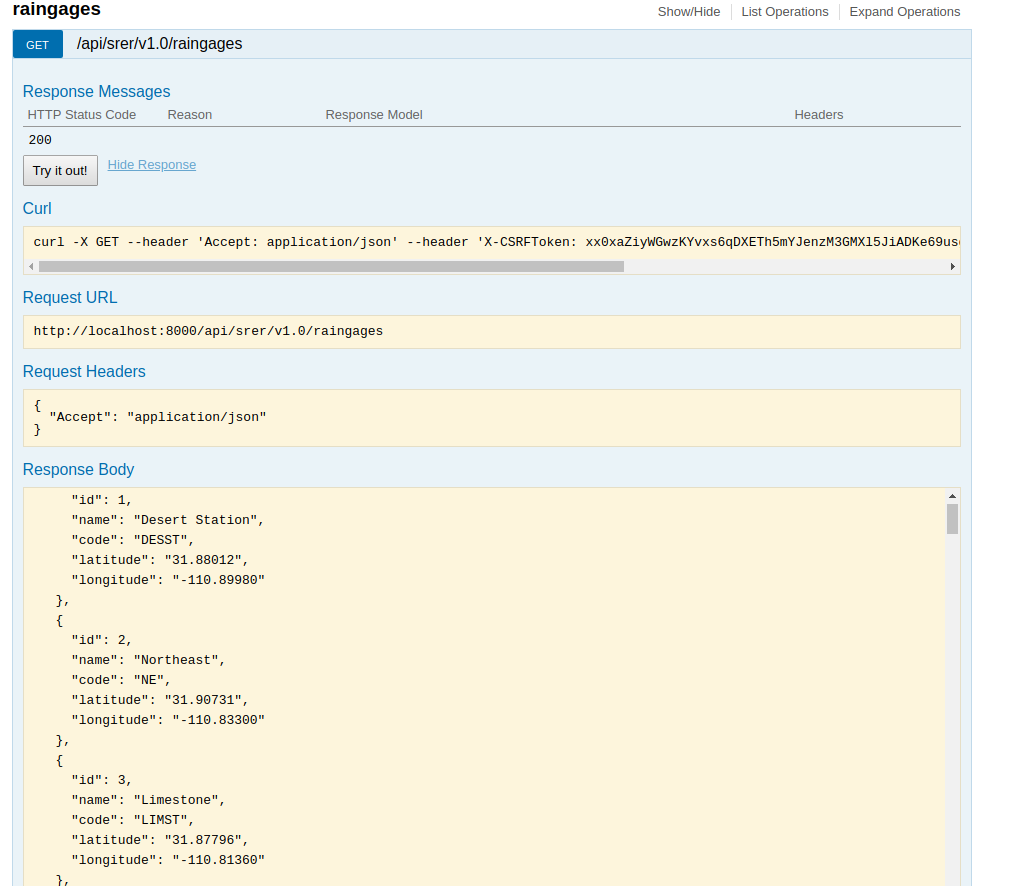
\includegraphics[width=\columnwidth]
  {./images/srer_rest_raingage_list.png}
  \caption{REST/SWAGGER Response}\label{f:srer_rest_raingage_list}
\end{figure}

\subsection{GraphQL API}
Similar to the REST/Swagger user interface, many GraphQL APIs allow the 
developer to enable a user interface that serves as the GraphQL API's 
documentation.  Figure~\ref{f:graphql_ui} shows an example of the GraphQL API 
interface.  At first glance, the GraphQL interface appears to not have nearly 
the amount of documentation that the Swagger equivalent has.  However, the 
input portion (left half) of the interface has autocomplete features and the 
user simple has to hit the space bar or start typeing in order to get guidance 
from the interface.

\begin{figure}[htb]
  \centering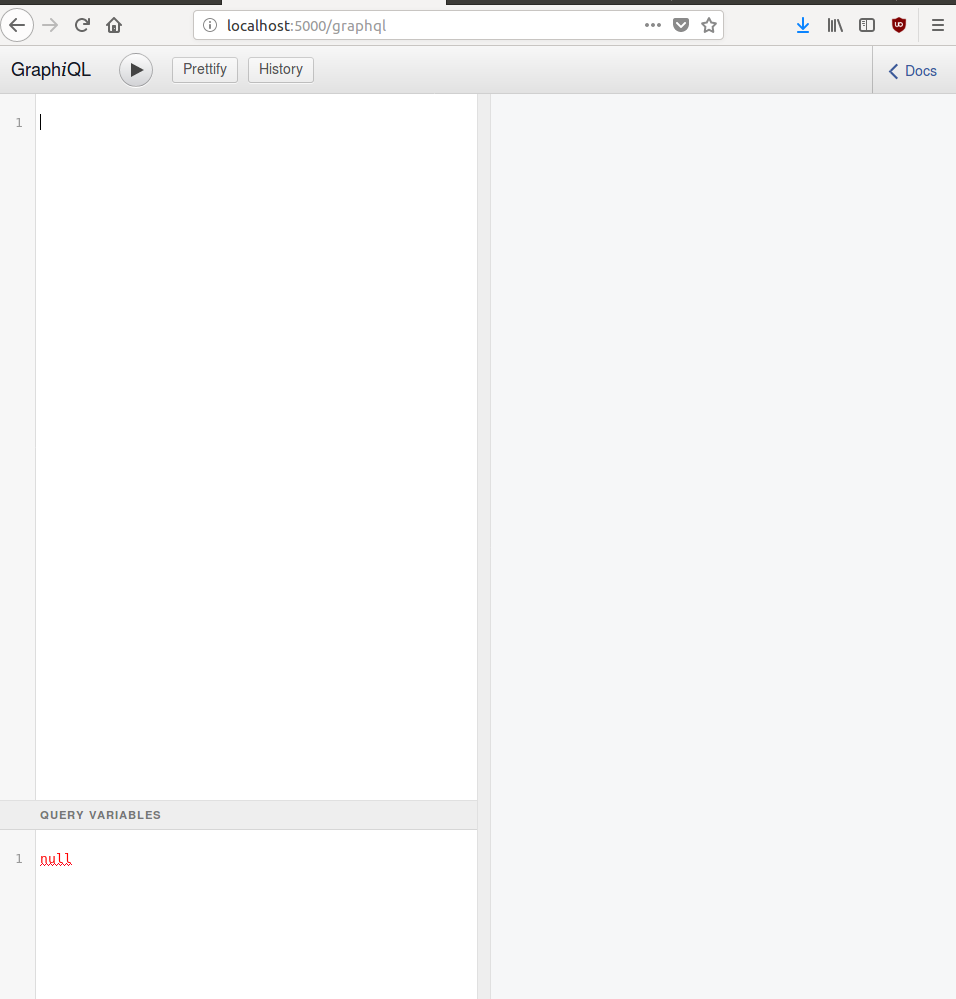
\includegraphics[width=\columnwidth]
  {./images/graphql_ui.png}
  \caption{GraphQL User Interface}\label{f:graphql_ui}
\end{figure}

Figure~\ref{f:graphql_rgs} demonstrates an example of a query in the GraphQL 
UI that is used to request a list of objects, in this case, all raingages.  
The left half of the user interface is where the query is created.  The 
interface behaves similarly to many itegrated development environments 
(IDE) by being aware of the underlying data model and query request 
parameters.  Consequently, as the user is developing the query, the UI 
provides autocomplete features that help expedite query development.

\begin{figure}[htb]
  \centering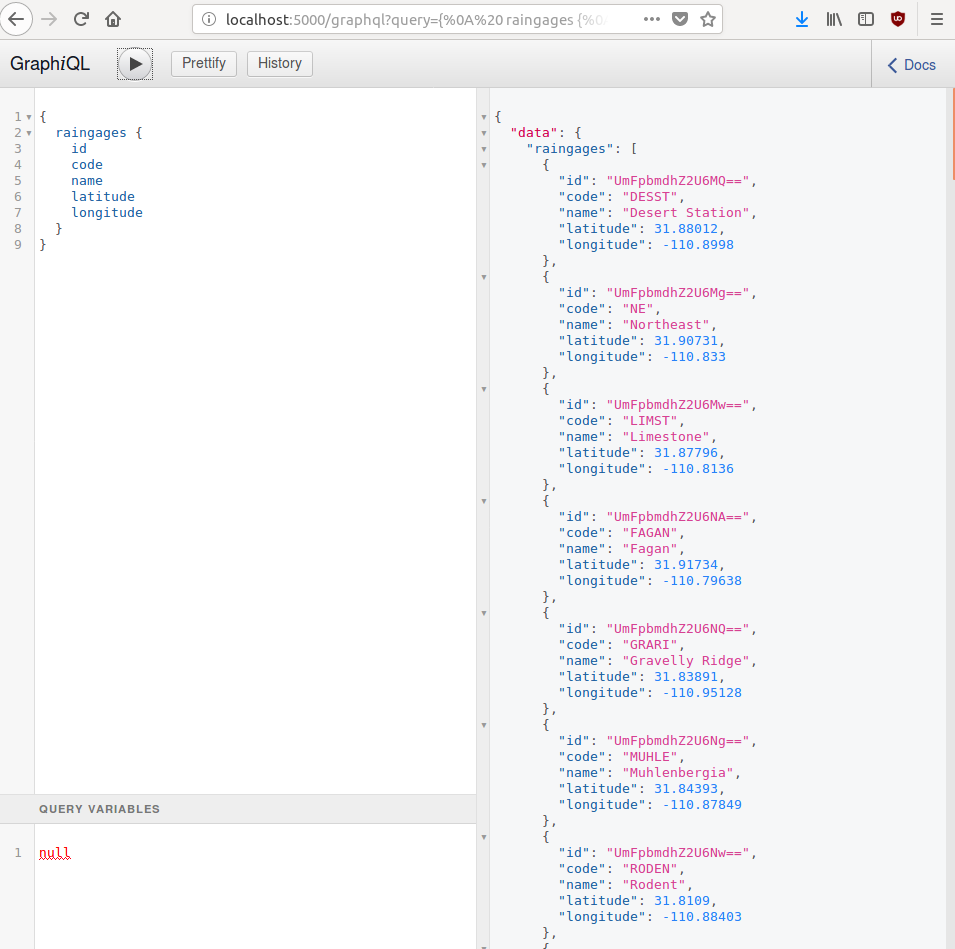
\includegraphics[width=\columnwidth]
  {./images/graphql_rgs.png}
  \caption{GraphQL UI Query Example}\label{f:graphql_rgs}
\end{figure}

The query results are JSON data packet that is a list of raingage objects 
including attributes for each raingage.  As with many other API's, this data 
packet can be consumed by a wide variety of clients including other web 
applications or thicker desktop clients like the statistical package R.

REST based API's are typically developed with create, retrieve, update and 
delete (CRUD) actions.  GraphQL APIs offer the same type of actions, but 
not in the same format.  Due to time constraints demonstration of those 
actions is outside of the scope of this paper.

\section{Service Comparison}
New tools like GraphQL have an appeal to developers because they are new tools 
and provided entertaining opportunities to learn something new.  However, it 
is important to validate the benefit of new tools by developing comparisons 
and measures against existing tools in order to assess qualitative attributes 
based on observed data and analysis.

Figures~\ref{f:comparison-table} 
and~\ref{f:comparison-graph}\cite{hid505Vzquez2017} demonstrate performance 
metrics and analysis based on their research.  Their results indicate that 
GraphQL may have better performance rates.

\begin{figure}[htb]
  \centering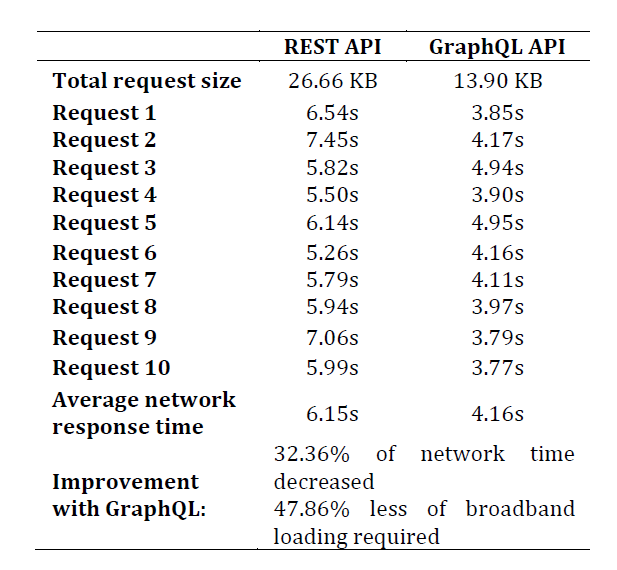
\includegraphics[width=\columnwidth]
  {./images/network-response-times-table.png}
  \caption{GraphQL/REST Comparision}\label{f:comparison-table}
\end{figure}

\begin{figure}[htb]
  \centering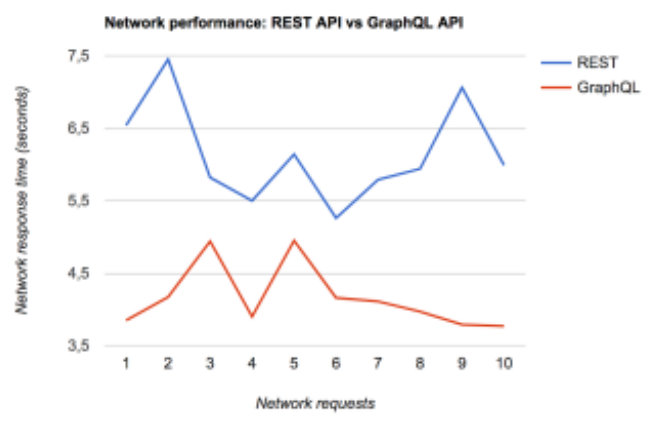
\includegraphics[width=\columnwidth]
  {./images/network-response-times-graph.png}
  \caption{GraphQL/REST Comparision}\label{f:comparison-graph}
\end{figure}

In hopes of providing more effidence related to GraphQL performane in 
comparison to REST performance.  A simple load test was created to test 
the REST API developed for this project against the GraphQL API created also 
created for this project.

The test environment consisted of:
\begin{enumerate}
\item HP Spectre X360 Laptop with 16 GB of RAM
\item Intel i7 Processor
\item Ubuntu 16.04 Operating System
\item PostgreSql 9.5 Database Server
\item Python 3.6.4
\item Django 2.0.3
\item Locust Python load testing API and command line tool
\item Graphene and Dango-Grapql plugins were used to create the GraphQL API
\item Django Rest Framework was used to create the REST API
\end{enumerate}
The source code repository for this project provides more detail on APIs and 
Python libraries used to develop the interface.

The load test was simple in each case, simulate 100 users, spawning 5 users 
per second, for 10 minutes.  The Python load testing tool, Locust, was used 
to run each test under the described parameters and the web interface in 
Locust provided summy graphics showing the results of the test.

Figure~\ref{f:f:graphql_requests} and Figure~\ref{f:graphql_response} 
demonstrate simple load-tests run against the GraphQL API developed for this 
project.

\begin{figure}[htb]
  \centering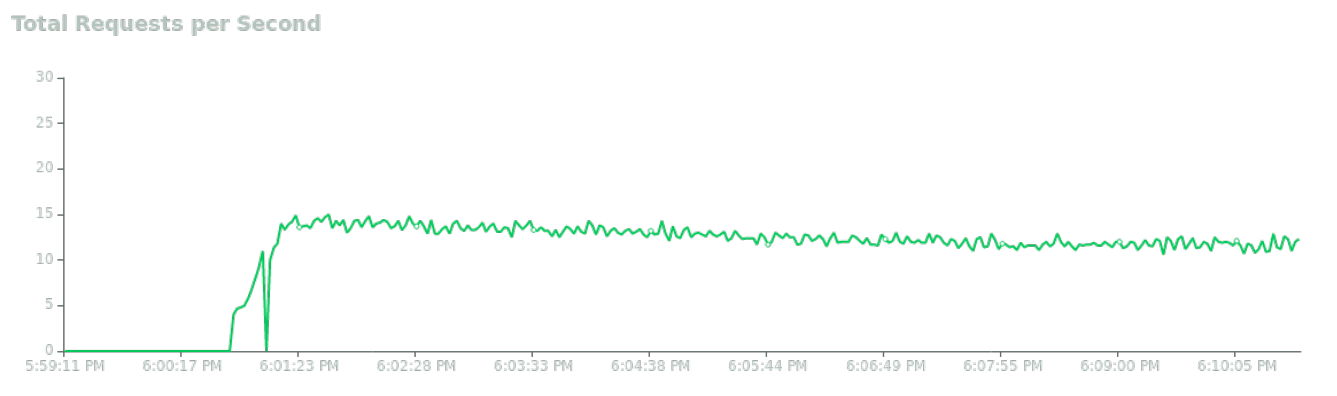
\includegraphics[width=\columnwidth]
  {./images/graphql_requests.png}
  \caption{GraphQL Total Requests per Second}\label{f:graphql_requests}
\end{figure}

\begin{figure}[htb]
  \centering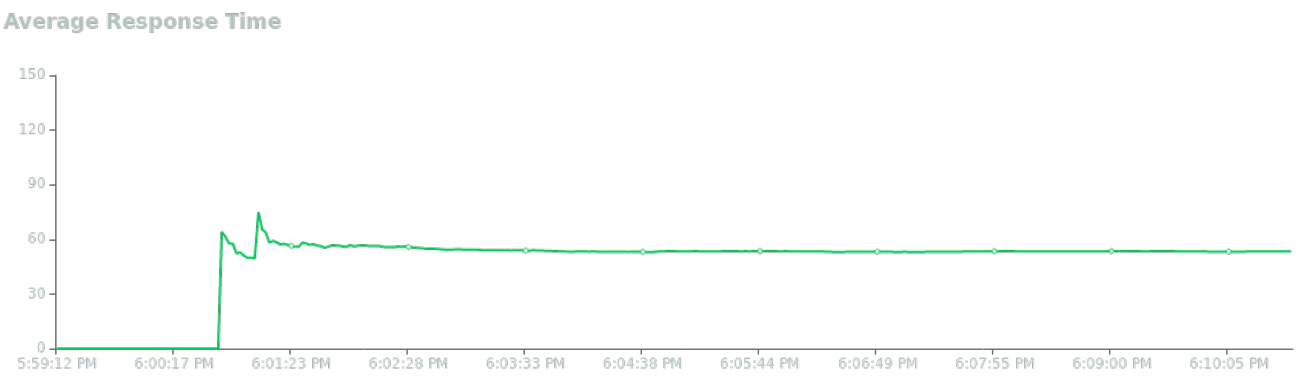
\includegraphics[width=\columnwidth]
  {./images/graphql_response.png}
  \caption{GraphQL Average Response Time}\label{f:graphql_response}
\end{figure}

Figure~\ref{f:rest_requests} and Figure~\ref{f:rest_response} show the results 
of the same test run against the REST API for the web application.

\begin{figure}[htb]
  \centering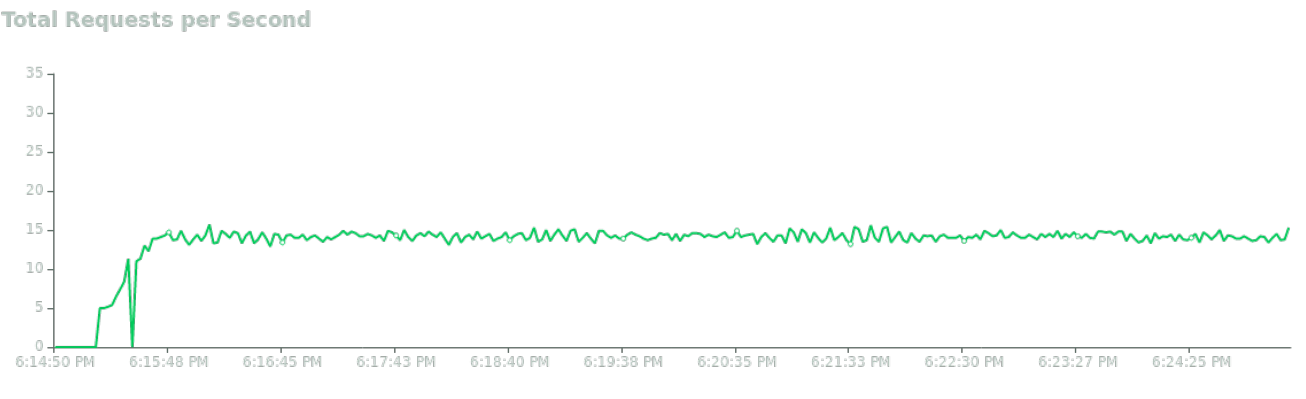
\includegraphics[width=\columnwidth]
  {./images/rest_requests.png}
  \caption{REST Total Requests per Second}\label{f:rest_requests}
\end{figure}

\begin{figure}[htb]
  \centering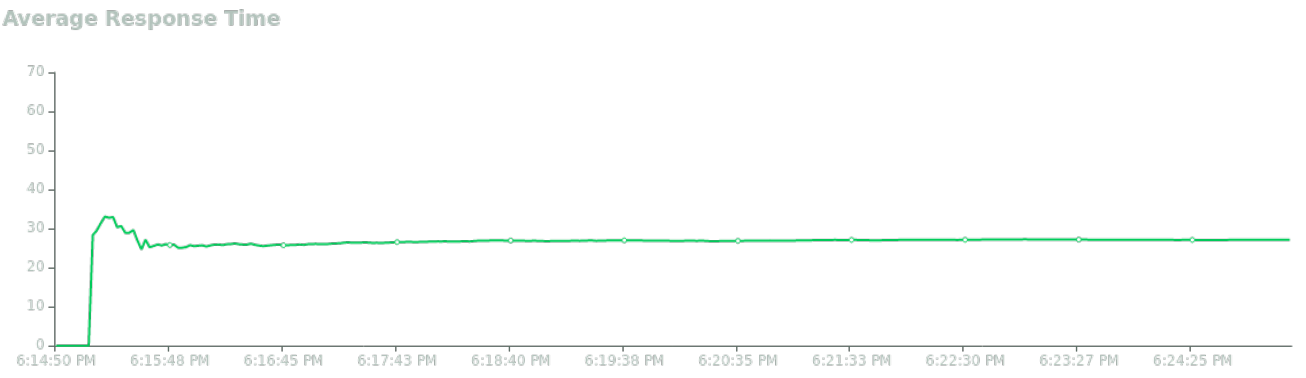
\includegraphics[width=\columnwidth]
  {./images/rest_response.png}
  \caption{REST Average Response Time}\label{f:rest_response}
\end{figure}

Contrary to expectations the test demonstrates that the response times for the 
REST web service are lower than for the equivalent GraphQL service.  However, 
given that the particular test is simplistic and there could be many other 
factors affecting the test, there is no evidence in this study to make 
qualitative statements about the performance of eith GraphQL or REST.  A more 
robust examination of the demo application and a rigorous load-testing design 
would be required in order to develop accurate insights into performance 
differences between the two technologies.

\section{Cloud Infrastructure}
In order to provide further proof-of-concept that the application and its 
respective data services and data are viable as web services in a 
near-production setting, a production like environemtn for the application 
was created using Amazon's Elastic Beanstalk (EB) cloud infrastructure.  This 
paper does not serve as a tutorial on how to create an Amazon AWS account nor 
will we offer a complete tutorial on how to create an EB application.  
However, the following outlines and describes the experience and findings in 
the process of converting this application to a EB cloud-hosted application.

\subsection{AWS Elastic Beanstalk}
``AWS Elastic Beanstaok is an easy-to-use service used to deploy and scale web 
applications developed in programming languages like Java, Python, PHP, and 
others.''\cite{AWSEB2018}

The proceedure for creating and deploying an AWS EB application is relatively 
straight forward.  A developer can either initialize an application using the 
EB web console or, if the user installs the EB command-line-interface (CLI) 
the application can be initialized locally.  The developer can chose from 
several programming languages and specifies the programming language during 
project initialization.  The initialization process requires the developer to 
create deployment configuration data so that AWS EB knows what programming 
language and what type of application is to be deployed and served over the 
internet.  The application can exist locally before deployment and once 
properly  configured the application can be deployed and almost run on first 
deployment.  

However, most web applications rely on a backend database server like 
PostgreSql or MySQL.  Amazon offers database servers throught its 
Relational Database Service (RDS)\cite{RDS2018}.  The application's 
database is created after the application is initialized and after EB knows 
about the application.  The database is added as a RDS component to the EB 
application via online configuration.  Once RDS is configured for the 
application, the appliation code has to be modified so that the codes has 
database connection information that applies to the production environment 
(EB) or local development environment.

A third feature that EB offers that facilitates development and deployment of 
web applications to a cloud based infrstructure is how EB handles static 
files.  Web applications typically have many static files like images, 
cascading style sheets, javascript files and more.  Those files tend to not 
change as frequently as application code does and ideally should be served 
seperately by a separate serve for security and efficiency reasons.  However, 
dealing with that type of deployment can require quite a bit of time and 
increases complexity.  EB has an elegant solution for this.  A web 
application, once configured and initialized is automatically provide and 
Amazon S3 Bucket\cite{S3Bucket2018}.  Amazon EB, automatically creates a 
storage location for the application's static files, copies those files when 
needed, to the storage location and serves those files for the web 
application.  Typically, in a non-EB environment that is work the programmer 
has to develop and maintain.

\section{Conclusion and Findings}
The goal of this paper and project was, using precipitation and raingage data 
develop two different Web APIs and compare those APIs.  The first API uses 
REST to create, read, update and delete data (CRUD), while the second API used 
GraphQL to offer the same CRUD functions.  Due to time constraints both APIs 
were developed only for read and a simplified query operations.  After both 
API's were developed a very simple benchmark test was executed against the 
endpoints the query for all raingage data in both APIs (REST, GraphQL).  A 
simple benchmark comparison was developed to demonstrating request response 
rates for each API.

\subsection{REST and GraphQL}
The load tests cited earlier in the paper that the application's REST services 
tended to handle requests better than the GraphQL services.  However, the 
Vazquez-Ingelmo, Cruz-Benito, Garcia-Palvo\cite{hid505Vzquez2017} research 
demonstrates that GraphQL can produce improve request-response rates than 
REST.  Overall, there are many things to consider when deciding to pick 
between the two web-service methods.  Once possible consideration is caching.  
Because REST services tend to be more static in form that GraphQL services it 
may be easier to implement caching when needed for larger-scaled web-APIs.

\subsection{Cloud Deployment}
There were multiple reasons for chosing Amazon's Elastic Beanstalk as the 
deployment platform for the live version of the application.  The possible 
deployment platforms to chose from where Heroku\cite{Heroku2018} and, as 
mentioned Amazon's Elastic Beanstalk.  Heroku offers a simplified deployment 
environment that, as long as the project structure complies with one of the 
Heroku prescribed project structures, makes deployment a very simple process.  
Also, Heroku has excellent recovery process in place so that if an applcition 
is deployed and there is a failure in the deployment process, Heroku stops the 
deploy and allows the existing deployment to continue running.  However, 
Heroku has a notably higher fee structure, which was the primary reason for 
choosing Amazon's Elastic Beanstalk.  

Amazon's Elastic Beanstalk has a higher learning-curve than Heroku, but once 
the project is configured properly and deployed, work flow for making and 
committing application changes becomes streamlined.  Also, Django applications 
are known for being easy to start in development, but difficult to deploy for 
testing and production.  In particular a significant amount of work has to be 
done in order to make static files available.  Elastic Beanstalk automatically 
handles static file deployment and serving static files if the application is 
configured propertly.  After the developer completes the proper configuration, 
Elastic Beanstalk takes care of the rest with regrads to static files.

Another finding worth noting, while creating a cloud-based application 
like this one, was how to handle getting initial data sets into the 
application.  This application relied upon data from the Walnut Gulch 
Experimental Watershed and the Santa Rita Experimental Range. SRER 
precipitation data set was the largest and consisted of approximately 30,000 
records, which is not a large data set.  However, importing even 30,000 
records proved to be resource intensive during the initial import.  WGEW 
precipitation data set consisted of over 300,000 data points.  This was a 
significant number to handle and proved problmetic during the deployment of 
after created API features related to WGEW.  Initially, data import was 
handled during each deployment of the application.  The databases tables were 
initialized and populated during each deployment.  This was considered 
acceptable until all of the initial data was loaded and worked while the SRER 
data were the only data in the database.  However, once the WGES data 
(300,000) records were incorporated into the deployment process, the 
deployment did not execute properly and left the application in a 
non-recoverable state in Amazon's Elastic Beanstalk.  Fortunately, recovering 
from such a state and in the context of this project was a straight-forward 
process requiring re-setting some Elastic Beanstalk settings, removing the 
application from Elastic Beanstalk and re-deploying to a newly created 
application environment on Elastic Beanstalk.  However, this meant figuring 
how to deploy the initial data sets since they still needed to be 
incorporated into the live application.  

Elastic Beanstalk also provides remote database access to backend database 
servers being used as part of web applications like this one.  Consequently, 
a secured, direct connection was created between the devlopment workstation 
and the production database where batch SQL-imports were used to complete the 
transfer of the initial data sets.  This method ultimately proved to be a 
faster method than the application deployment method.

Finally, as of the completion of this paper the total costs incurred on 
Amazon's Elastic Beanstalk, which includes the deployed web application 
and Amazon S3 Bucket for storing static files and a PostgresQL database 
server with initial data import, and a few web requests to confirm the 
application is running amount to just under five dollars.  The web 
application can be reviewed by opening a web browser to www.earthapi.net.  
A video documenting the AWS Elastic Beanstalk instance and console can be 
views at http://www.acatejr.com/cc.

\begin{acks}
The authors would like to thank Dr.~Gregor~von~Laszewski for his support 
and suggestions to write this paper.  The authors would also like to thank 
the following people.  Dr.~Mitch~McLaran of the University of Arizona's School 
of Natural Resources and The Environment for providing access and support of 
the SRER website.  Craig Wissler of the University of Arizona's School of 
Natural Resources and The Environment for providing feedback on related to the 
SRER data.  Dr.~David~Goodrich and Dr.~Phil~Heilman, both from the United 
States Deparment of Agriculture's Southwest Watershed Research Center, for 
providing support and access to the Walnut Gulch Experimental Watershed 
website and data.
\end{acks}

\bibliographystyle{ACM-Reference-Format}
\bibliography{report} 
